\documentclass[10pt,a4paper]{article}
%\usepackage[latin1]{inputenc}
\usepackage{listings}
\usepackage{amsmath}
\usepackage{amsfonts}
\usepackage{amssymb}
\usepackage{graphicx}
\usepackage{multirow}
\usepackage{tikz}
\usepackage[left=2.00cm, right=3.00cm, top=2.00cm, bottom=2.00cm]{geometry}
\usepackage{bm}
\usepackage[colorinlistoftodos]{todonotes}

\definecolor{on_bckgrd}{HTML}{F6BCB2}
\definecolor{off_bckgrd}{HTML}{A4D5EA}

%--- Variables ---%
\providecommand{\ve}[1]{{\bm {#1}}} %
\providecommand{\mat}[1]{{\bm {#1}}} %

%--- Operators ---%
\providecommand{\abs}[1]{\lvert{#1}\rvert}%
\providecommand{\norm}[1]{\left|\left|{#1}\right|\right|} %
\providecommand{\normal}[2]{\mathcal{N} (#1, #2)} % FDP Gauss
\providecommand{\dotp}[2]{\langle #1, #2 \rangle}
\providecommand{\mean}[1]{ \mathcal{E} \{#1\} }
\providecommand{\est}[1]{{\widehat{#1}}}
\providecommand{\cov}[1]{{\mathrm{cov}\left({#1}\right)}}
\providecommand{\corr}[1]{{\mathrm{corr}\left({#1}\right)}}
\providecommand{\vect}[1]{{\mathrm{vec}\left({#1}\right)}}
\DeclareMathOperator*{\argmin}{arg\,min}
\DeclareMathOperator*{\argmax}{arg\,max}
\DeclareMathOperator*{\diag}{\mathrm{diag}}
\DeclareMathOperator*{\Diag}{\mathrm{Diag}}
\providecommand{\geodist}[2]{{\ensuremath{d_g}}\{#1,#2\}}

%--- Other ---%
\newcommand{\Real}{\mathbb{R}}
\newcommand{\Complex}{\mathbb{C}}
\newcommand{\Natural}{\mathbb{N}}
\newcommand{\T}{\textsf{T}}
\newcommand{\x}{\times}

%--- Text modifiers ---%
\providecommand{\red}[1]{\textcolor{red}{#1}}
\providecommand{\blue}[1]{\textcolor{blue}{#1}}
\providecommand{\black}[1]{\textcolor{black}{#1}}
\providecommand{\green}[1]{\textcolor{green}{#1}}
\providecommand{\magenta}[1]{\textcolor{magenta}{#1}}

\providecommand{\mat}[1]{{\bm {#1}}}


\newcommand{\cpd}[0]{\textit{copy-draw}}
\newcommand{\cpdt}[0]{\textit{copy-draw}~test}
\newcommand{\patient}[2]{$S_{#1}^{#2}$}

%\title{Data-driven identification of acute and chronic cortical neural-markers for characterization of Parkinson's diseases symptoms}
\title{Data-driven characterization of cortical neural markers in acute and chronic stages of DBS treatment for Parkinson's disease}
% non-stationarity
% acute and chronic
%
%
%
\begin{document}
\maketitle
\listoftodos

\begin{abstract}

\begin{itemize}
\item Motor performance decoding from EEG features
\item Are the identified features the same as in CSP for classifying DBS ON/OFF?
\item How are the intra-trial dynamics?
\item How are the intra-session dynamics?
\item Non trivial decoding (compare to SSD)
\item Stationarity of relevant components across sessions
\end{itemize}
\end{abstract}

\section{Introduction}

\section{Methods}
\subsection{Motor paradigm - \cpdt}
\subsection{Quantification of motor performance}
\subsection{Decoding of PD-relevant motor performance}

Based on the assumption that relevant NM can be found in cortical and subcortical signals, it can be hypothesized that underlying EEG sources may contain relevant information about NMs for PD.  Following, we will describe how these informative oscillatory sources can be recovered from overlapping confounds and noisy EEG signals in a short-timescale, single-trial basis. 

\subsubsection{Forward model of EEG generation}
\label{par:modeling}
%\begin{figure}[h!]
Due to volume conduction, non-invasive imaging techniques, as EEG, measure electrical brain activity generated by superimposed hidden brain sources. In general, the properties of such superposition is linear, thus, it can be described as a linear combination of neural generators, which can be modeled as follows.

Let $\mat{X}\negmedspace\in\negmedspace \Real^{N_c \times N_t}$ be a multivariate variable to describe data of brain activity measured in the EEG sensor space, where $N_t$ is the number of time samples and $N_c$ the number of sensors. Furthermore, let $\mat{S} \negmedspace\in\negmedspace \Real^{N_s \times N_t}$ describe the time course of $N_s$ neural sources, where $N_s$ describes the number of hidden neural sources considered. Then, the general EEG generative model can be written as: 
\begin{align}\label{eq:genModel}
\mat{X}=\mat{A}\,\mat{S} + \mat{E} \;.
\end{align} 
In this model, matrix $\mat{A}\negmedspace\in\negmedspace \Real^{N_c \times N_s}$ describes the projection of the sources to the sensor space, where the columns of $\mat{A}$, $\ve{a} \negmedspace\in\negmedspace \Real^{N_c}$, are referred to as \emph{spatial patterns}. Furthermore, the matrix $\mat{E}$ contains spatially and temporally uncorrelated noise to model measurement noise. 

An estimation of the time-course of a source component, i.e.\ $\hat{\ve{s}}$, can be extracted from the measurements by way of a \emph{spatial filter} $\ve{w} \in \Real^{N_c}$, which projects the data from sensor space into source space. Thus we have $\hat{\ve{s}} = \ve{w}^\top\mat{X}$.
%A source component $\hat{\ve{s}}_X=\ve{w}^\top\mat{X}$
%can be extracted from the time course of the sensor data by applying a  spatial filter $\mat{w}\negmedspace\in\negmedspace\Real^{N_c \times 1}$, which projects data from the sensor space to the source space. 
For many problems, such a spatial filter $\mat{w}$ is not known a priori and must be estimated from the data. However, once a spatial filter (or an entire set thereof, denoted by $\mat{W} \in \Real^{N_c \times N_s}$, where each column $\ve{w}$ represents a single spatial filter) has been obtained, an estimate of the corresponding spatial patterns can be computed via the relation $ \hat{\mat{A}} = \mat{C} \mat{W} \left( \mat{W}^\top \mat{C} \mat{W} \right)^{-1} $, where $\mat{C} \in  \Real^{N_c \times N_c} $ denotes the spatial covariance matrix of the data $\mat{X}$. See \cite{haufe2014interpretation} for further details on the relation between spatial filters and spatial patterns.  

\subsubsection{Common Spatial Patterns --- CSP}

\subsubsection{Source Power Co-modulation --- SPoC}
\label{par:spoc}
The source power co-modulation (SPoC) method introduced in~\cite{dahne2014spoc} utilizes a supervised regression approach in order to estimate a set of spatial filters $\mat{W}$. The method assumes that the recorded data $\mat{X}$ has been pre-filtered to a narrow frequency band, which contains the oscillatory source of interest. 

Based on data of multiple epochs $e$, a filter $\mat{w}$ is optimized such that the power of an epoch $\Theta_x(e) = \operatorname{var}[\hat{\ve{s}}](e)$ of the spatially filtered data $\hat{\ve{s}}=\mat{w}^\top\mat{X}$, maximally covaries with a known, epoch-wise defined univariate target variable $z(e)$. For the sake of simplicity in the notation, $\hat{\ve{s}}$ will be noted as $\ve{s}$, hereafter.
 
%\end{align}
It can be shown that solving the optimization problem described above, is equivalent to solving the following generalized eigenvalue problem
\begin{align}\label{eq:eig_spoc}
\mat{C}_z\mat{W} = \mat{\Lambda}\mat{C}\mat{W}
\end{align}
where $\mat{C}_z = \left<\mat{C}(e)z(e)\right>$, $\mat{C} = \left<\mat{C}(e)\right>$, and $\left<\mat{C}(e)\right>$ and $\left<\mat{C}(e)z(e)\right>$ are, respectively, the weighted covariance and covariance of $\mat{X}$, averaged across epochs $e$: $\mat{C}(e) = \mat{X}(e)\mat{X}(e)^\T$; and $\mat{\Lambda} \in \Real^{N_c\times N_c}$ is a matrix containing the corresponding eigenvalues in the main diagonal.

Given a spatial filter $\mat{w}_{tr}$ determined on training data $tr$, the true target variable $z$ can subsequently be approximated on a single-trial basis for unseen test data ($te$) epochs $\mat{X}_{te}$ via $\hat{z}(e) = \operatorname{var}[\mat{w}_{tr}^\top\mat{X}_{te}(e)]$. 


\section{Experimental setup}
\subsection{Patients}

\subsection{Study design}
Three PD patients (P1, P2, and P3) were bilaterally implanted in the STN with directional DBS electrodes (Vercise Cartesia \texttrademark Boston Scientific, Marlborough, MA, USA). After implantation, DBS leads were kept externalized during three days following surgery (D1, D2, and D3). On day four, leads were internalized and pulse generator (IPG) was implanted. Each patient participated in 5 experimental sessions, as depicted in Figure \ref{fig:sessions_overview}. In four of the five sessions, the copy-draw task was executed under different conditions:
\begin{itemize}
\item \textit{Pre-session}: An EEG-only session, several days prior to implantation surgery.
\item \textit{Acute sessions D2 and D3}: On days two and three after DBS electrode implantation, the copy-draw task was executed under varying stimulation regimes with concurrent EEG and LFP recordings.
\item \textit{Chronic session}: During the first control-visit after DBS system implantation (at least one month thereupon), patients participated in a final EEG session, where the copy-draw task was executed under varying DBS and medication conditions.
\end{itemize}

\subsection{Experimental session}
Each copy-draw session was structured in the form of \text{blocks}, where each block comprised 12 trials. For each session, a number of at least 8 \textit{blocks} were executed, in order to guarantee enough data samples to reliably train the SPoC model. Sessions D2 and D3 of patient P3 were left out of further analysis, due to their premature interruption, at 5 and 6 blocks, respectively.

Furthermore, dopaminergic medication was suspended at least 12 hours before each session. During the sessions, patients were allowed to take the suspended medication (Madopar LT, T, or Stalevo) according to the level of discomfort occasioned by PD symptoms.

\begin{figure}[h!]
\centering
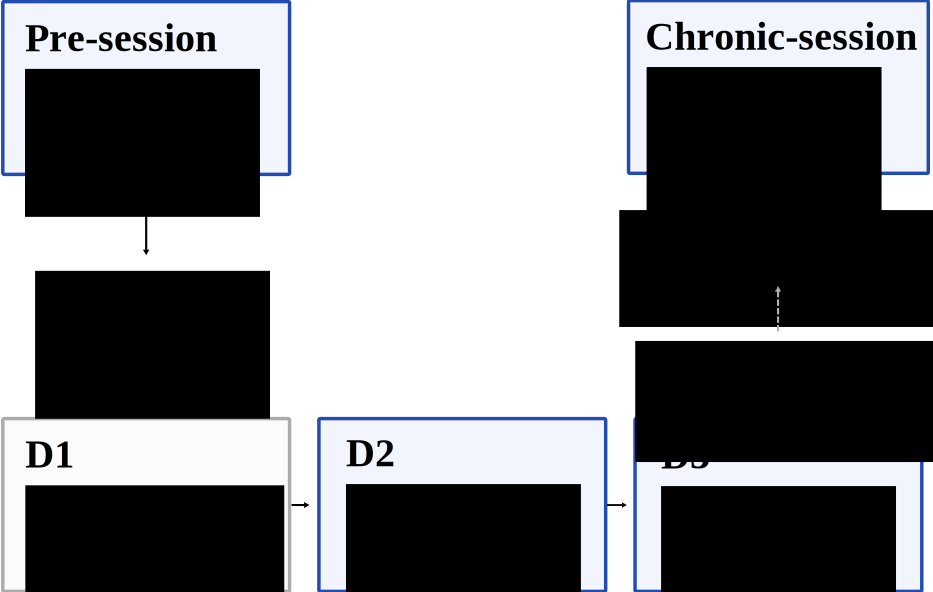
\includegraphics[width=0.45\textwidth]{figures/all_sessions}
\caption{Overview of all experimental sessions carried out by the patients.}
\label{fig:sessions_overview}
\end{figure}

\subsection{Signal acquisition}
\subsubsection{EEG-only sessions -- Pre-/ and chronic sessions}
EEG signals were recorded from 64 passive Ag/AgCl electrodes (EasyCap GmbH, Germany) placed according to the extended 10-20 system. Impedances were kept below 20\,k$\Omega$. All channels were referenced against the nose during recording. The EEG signals were registered by BrainAmp DC amplifiers (Brain Products GmbH, Germany) at a sampling rate of 1\,kHz, with an analog lowpass filter of 250\,Hz applied before digitization.

\subsubsection{Acute sessions with externalized DBS electrodes}
EEG signals were recorded from a variable number of the same passive Ag/AgCl electrodes placed according to the 10-10 system, using an EEG cap with 128 electrodes. The EEG electrodes chosen for recording were carefully selected, so as to avoid injured tissue. Areas avoided corresponded to fronto-central, central, and centro-parietal electrodes, slightly asymmetrical, depending on the side from which the leads were externalized, as illustrated in Figure \ref{fig:paradigm_layout}. Impedance of the selected electrodes were kept below 20\,k$\Omega$.

DBS electrodes were connected the NeuoOmega system (AlphaOmega, Israel), were DBS was delivered according to each condition

\begin{figure}[h!]
\centering
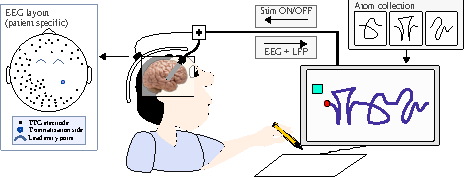
\includegraphics[width=0.8\textwidth]{figures/paradigm_layout}
%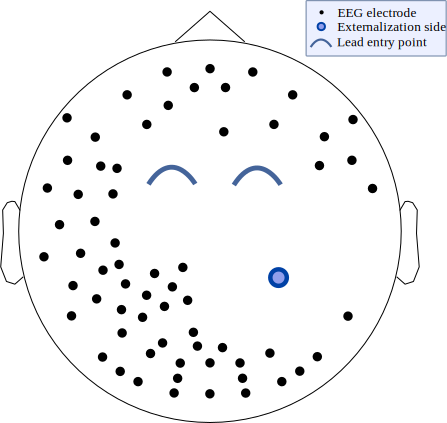
\includegraphics[width=0.4\textwidth]{figures/electrode_layout}
%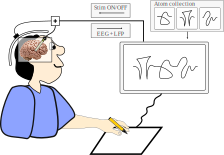
\includegraphics[width=0.5\textwidth]{figures/paradigm}
\caption{Right: Illustrative EEG layout used for one of the patients. Electrodes were placed over the entire scalp, avoiding incision sites used for DBS electrode implantation and externalization. Left: Experimental setup used during days D1-D3. Concurrent EEG+STN-LFP signals were recorded during copy-draw Execution.}
\label{fig:paradigm_layout}
\end{figure}


\section{Results}
\def \allsessions {VPpcac_d2,VPpcac_d4,NEW,VPpcad_d2,VPpcad_d4,VPpcae_d4,NEW,VPpcaf_d2,
	VPpcaf_d3,VPpcaf_d4,NEW,VPpcag_d2,VPpcag_d3,VPpcag_d4,NEW,VPpcah_d2,NEW,
	VPpcaj_d2,VPpcaj_d3}

\subsection{Modulation of motor-performance}
Figure \ref{fig:behavioral_all} shows the $PL$ score achieved by the patients in all the sessions. Complex medication-stimulation interaction can be seen for many of the recordings. For example, in session P1-D2, DBS does not have an evident effect in motor performance at the beginning of the session, but after intake of dopaminergic medication, a clear difference between DBS ON and OFF may be observed

\begin{figure}
	\centering
	\def \subplotwidth {0.24\textwidth}
\begin{tabular}{cc|c}

\includegraphics[width=\subplotwidth]{./figures/histogram_labels/histogram_labels_VPpcac_d2}& & \includegraphics[width=\subplotwidth]{./figures/histogram_labels/histogram_labels_VPpcac_d4}\\
\includegraphics[width=\subplotwidth]{./figures/histogram_labels/histogram_labels_VPpcad_d2}& & \includegraphics[width=\subplotwidth]{./figures/histogram_labels/histogram_labels_VPpcad_d4}\\
& & \includegraphics[width=\subplotwidth]{./figures/histogram_labels/histogram_labels_VPpcae_d4}\\
\includegraphics[width=\subplotwidth]{./figures/histogram_labels/histogram_labels_VPpcaf_d2}& \includegraphics[width=\subplotwidth]{./figures/histogram_labels/histogram_labels_VPpcaf_d3}& \includegraphics[width=\subplotwidth]{./figures/histogram_labels/histogram_labels_VPpcaf_d4}\\
\includegraphics[width=\subplotwidth]{./figures/histogram_labels/histogram_labels_VPpcag_d2}& \includegraphics[width=\subplotwidth]{./figures/histogram_labels/histogram_labels_VPpcag_d3}& \includegraphics[width=\subplotwidth]{./figures/histogram_labels/histogram_labels_VPpcag_d4}\\
\includegraphics[width=\subplotwidth]{./figures/histogram_labels/histogram_labels_VPpcah_d2}& & \includegraphics[width=\subplotwidth]{./figures/histogram_labels/histogram_labels_VPpcah_d4}\\
\includegraphics[width=\subplotwidth]{./figures/histogram_labels/histogram_labels_VPpcaj_d2}& \includegraphics[width=\subplotwidth]{./figures/histogram_labels/histogram_labels_VPpcaj_d3}& \includegraphics[width=\subplotwidth]{./figures/histogram_labels/histogram_labels_VPpcaj_d4}\\
\end{tabular}
\caption{Motor performance}
\end{figure}




\subsection{Predictive cortical oscillatory components}
%\begin{figure}[h!]
\def \rSearchwidth {0.2}
\begin{tabular}{ccccc}

 & Pre session & D2 & D3 & Chronic \\
 P1 &
 \raisebox{-.5\height}{
 \includegraphics[width=\rSearchwidth\textwidth]{../code/output/rSearch_VPpcac_d0_len_test_auc.pdf}} &
 \raisebox{-.5\height}{
 \includegraphics[width=\rSearchwidth\textwidth]{../code/output/rSearch_VPpcac_d2_len_test_auc.pdf}} &
 \raisebox{-.5\height}{
 \includegraphics[width=\rSearchwidth\textwidth]{../code/output/rSearch_VPpcac_d3_len_test_auc.pdf}} & 
 \raisebox{-.5\height}{
 \includegraphics[width=\rSearchwidth\textwidth]{../code/output/rSearch_VPpcac_d4_len_test_auc.pdf}} \\
 
P2  &
\raisebox{-.5\height}{
\includegraphics[width=\rSearchwidth\textwidth]{../code/output/rSearch_VPpcad_d0_len_test_auc.pdf}} &
\raisebox{-.5\height}{
\includegraphics[width=\rSearchwidth\textwidth]{../code/output/rSearch_VPpcad_d2_len_test_auc.pdf}} &
\raisebox{-.5\height}{
\includegraphics[width=\rSearchwidth\textwidth]{../code/output/rSearch_VPpcad_d3_len_test_auc.pdf}} &
\raisebox{-.5\height}{
\includegraphics[width=\rSearchwidth\textwidth]{../code/output/rSearch_VPpcad_d4_len_test_auc.pdf}} \\

P3  &
\raisebox{-.5\height}{
\includegraphics[width=\rSearchwidth\textwidth]{../code/output/rSearch_VPpcae_d0_len_test_auc.pdf}} &
 & 
 &
 \raisebox{-.5\height}{
\includegraphics[width=\rSearchwidth\textwidth]{../code/output/rSearch_VPpcae_d4_len_test_auc.pdf}} \\
 
\end{tabular}
\end{figure}
\begin{figure*}
	\centering
\def \subplotwidth {0.24\textwidth}
\begin{tabular}{cc|c}
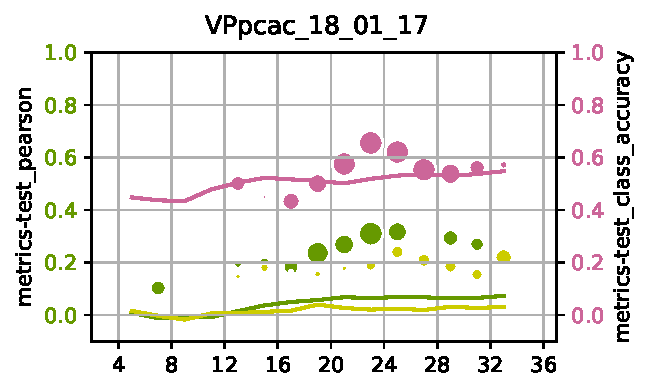
\includegraphics[width=\subplotwidth]{./figures/csp_spoc_incommon/bubble_csp_spoc_incommon_VPpcac_d2_nolegend}& & 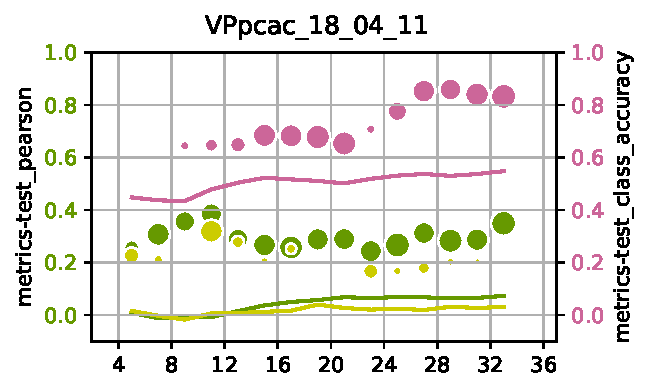
\includegraphics[width=\subplotwidth]{./figures/csp_spoc_incommon/bubble_csp_spoc_incommon_VPpcac_d4_nolegend}\\
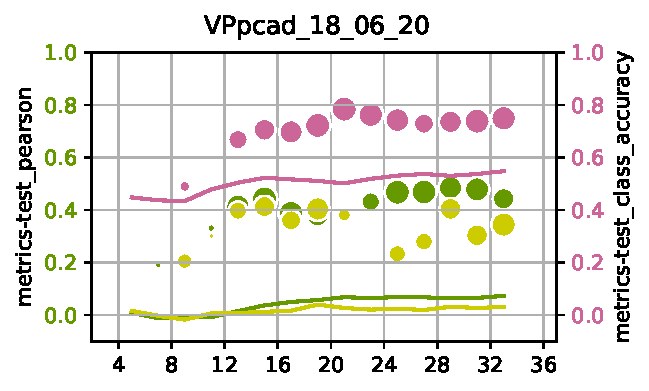
\includegraphics[width=\subplotwidth]{./figures/csp_spoc_incommon/bubble_csp_spoc_incommon_VPpcad_d2_nolegend}& & 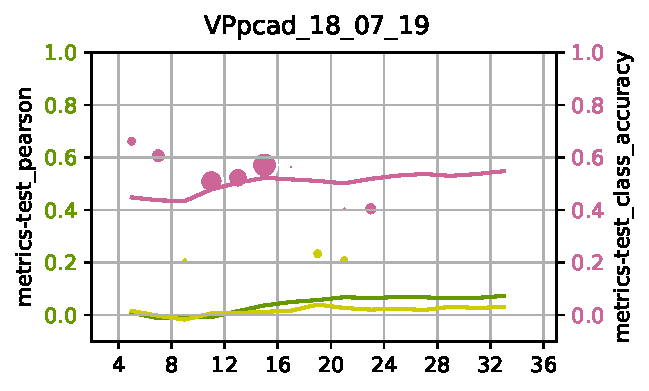
\includegraphics[width=\subplotwidth]{./figures/csp_spoc_incommon/bubble_csp_spoc_incommon_VPpcad_d4_nolegend}\\
& & 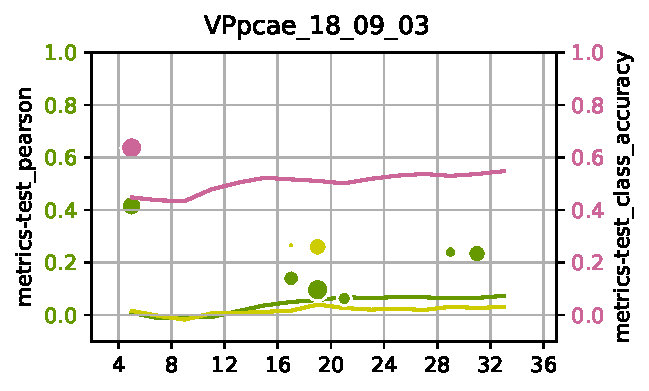
\includegraphics[width=\subplotwidth]{./figures/csp_spoc_incommon/bubble_csp_spoc_incommon_VPpcae_d4_nolegend}\\
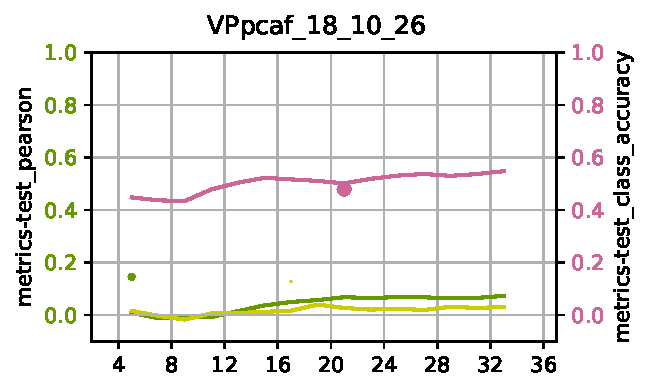
\includegraphics[width=\subplotwidth]{./figures/csp_spoc_incommon/bubble_csp_spoc_incommon_VPpcaf_d2_nolegend}& 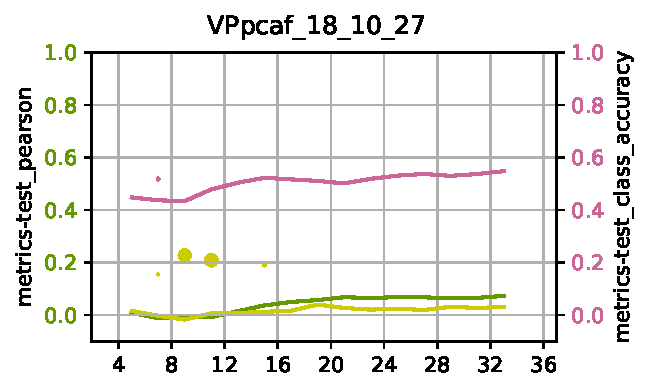
\includegraphics[width=\subplotwidth]{./figures/csp_spoc_incommon/bubble_csp_spoc_incommon_VPpcaf_d3_nolegend}& 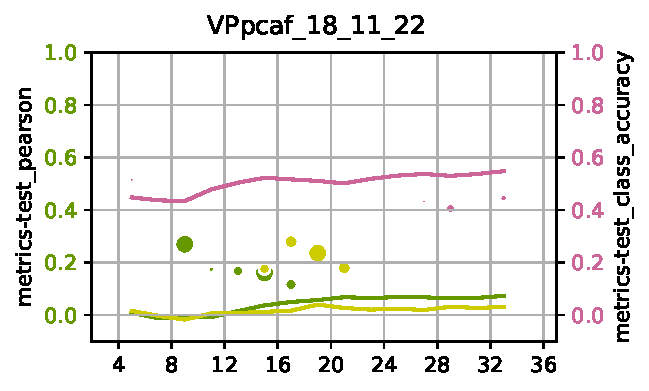
\includegraphics[width=\subplotwidth]{./figures/csp_spoc_incommon/bubble_csp_spoc_incommon_VPpcaf_d4_nolegend}\\
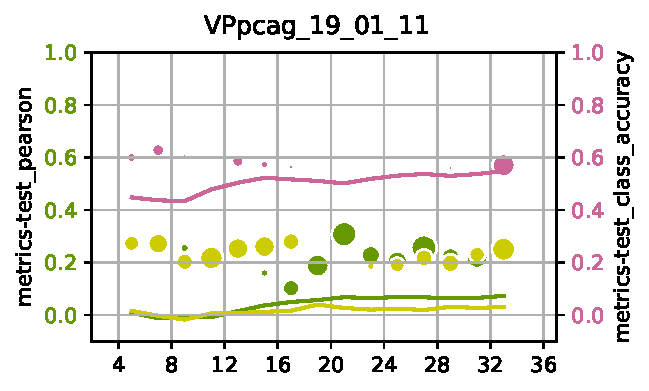
\includegraphics[width=\subplotwidth]{./figures/csp_spoc_incommon/bubble_csp_spoc_incommon_VPpcag_d2_nolegend}& 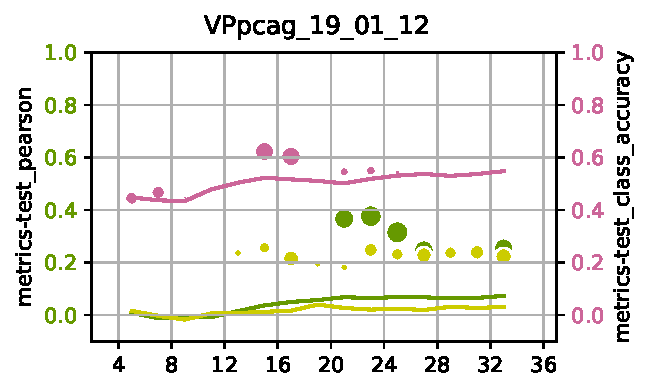
\includegraphics[width=\subplotwidth]{./figures/csp_spoc_incommon/bubble_csp_spoc_incommon_VPpcag_d3_nolegend}& 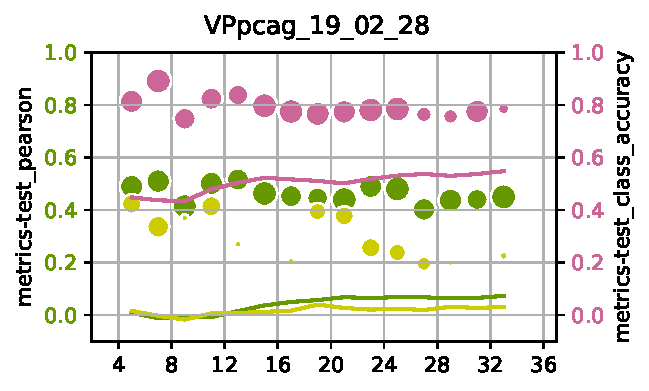
\includegraphics[width=\subplotwidth]{./figures/csp_spoc_incommon/bubble_csp_spoc_incommon_VPpcag_d4_nolegend}\\
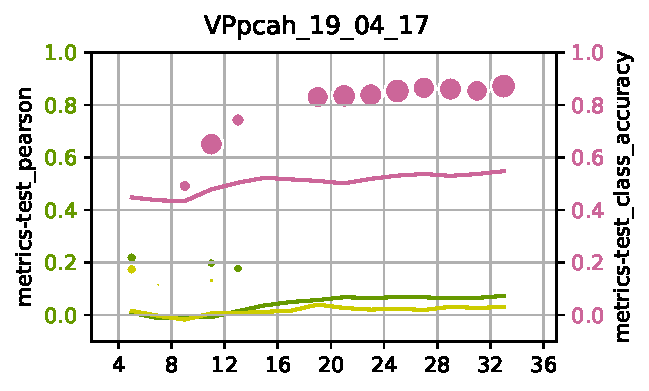
\includegraphics[width=\subplotwidth]{./figures/csp_spoc_incommon/bubble_csp_spoc_incommon_VPpcah_d2_nolegend}& & 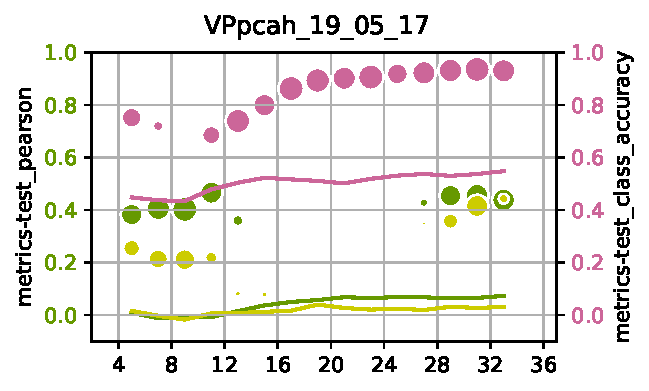
\includegraphics[width=\subplotwidth]{./figures/csp_spoc_incommon/bubble_csp_spoc_incommon_VPpcah_d4_nolegend}\\
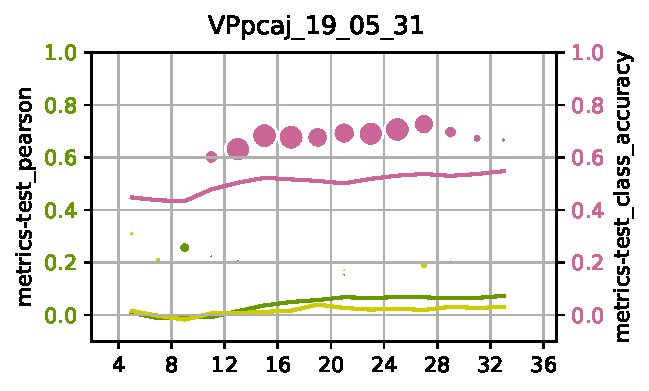
\includegraphics[width=\subplotwidth]{./figures/csp_spoc_incommon/bubble_csp_spoc_incommon_VPpcaj_d2_nolegend}& 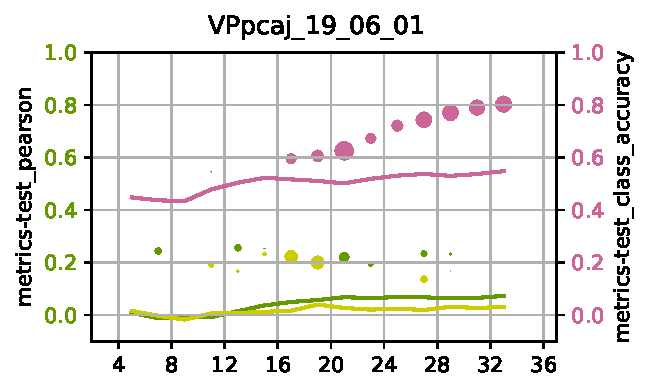
\includegraphics[width=\subplotwidth]{./figures/csp_spoc_incommon/bubble_csp_spoc_incommon_VPpcaj_d3_nolegend}& 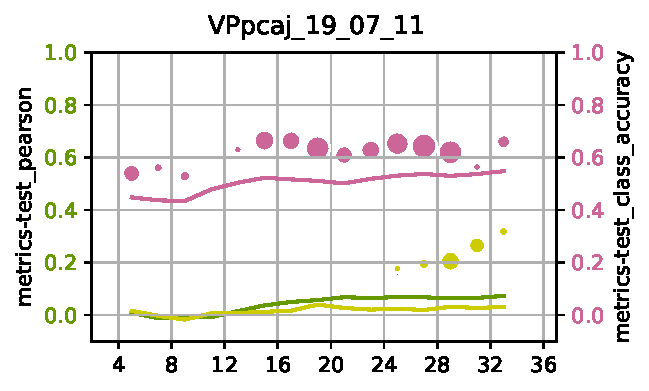
\includegraphics[width=\subplotwidth]{./figures/csp_spoc_incommon/bubble_csp_spoc_incommon_VPpcaj_d4_nolegend}\\
\end{tabular}
\caption{Motor performance}
\label{fig:decoding_performance_all}
\end{figure*}

\subsection{Spatio-temporal signatures}
In the following, the spatio-temporal signatures of the significant components identified for the chronic sessions will be presented. We have excluded the acute sessions from this analysis since the incompleteness of the EEG layout precludes the interpretation of the spatial patterns obtained. Here, we refer to spatio-temporal signatures as the set of spatial patterns identified by SPoC, as well as the corresponding averaged ERD/ERS.

From all the components obtained, we have manually discarded components that can be attribute to artifacts. The criteria used for distinguishing artifact vs non-artifact was based on the same criteria used in ICA, i.e., take into account the spatio-temporal-spectral signatures of the components \cite{MARAOrSimilarHowToIdentifyArtifacts}. For clarity, Figure \ref{fig:artifacts}, show an subset of components selected as artifactual.

Two type of components are found for \patient{1}{c}: 1) a lateralized parietal component extracted from the alpha band, and 2) a central component extracted from low and high beta band. The former might be attributed to attention process, whereas the latter suggest an underlying motor process. Also interesting the parietal pattern, contains a \cpdt-trial time-locked ERS which is also modulated by stimulation, with an enhanced ERS under DBS-on. 

For \patient{2}{c}, a much smaller amount of significant components was found. In this case, the spatial patterns are not clearly of neural origin, however, their spectral signature shows a narrow-band enhancement of the beta-band power.
\todo{analyze time series of second component, is this an eye artifact?}

For \patient{3}{c} \todo{Is this an eye artifact?}

\patient{4}{c}, show a significant temporal-parietal component found the alpha band. This component also shows a \cpdt-trial time-locked ERD. This component does not show a difference between conditions DBS-on and -off.

The spatio-temporal signatures found for \patient{5}{c} are noteworthy: Here, an average correlation of $\approx0.5$ was achieved for left-hemisphere pre-frontal components extracted from the theta-band, which are enhanced for DBS-on. This suggests that for this patient, the stimulated part of the STN might have abundant projections to the prefrontal cortex \todo{which part of the STN has projections on the prefrontal cortex?}. As this cortical area is known to modulate cognitive processes, this result might be interpreted as a modulation of motor performance by an underlying cognitive process, instead of a motor process. Simmilar cases have been reported before, where DBS-induced impulsivity would lead to an increased speed in these type of tasks \cite{IMPULSIVITY DBS}

In \patient{6}{c}, we found an stereotypical alpha-band oscipital component. This might indicate an underlying attention process. 

Finally, similar to the patterns found for \patient{5}{c}, for \patient{7}{c} we found a frontal (non-lateralized) theta-band component which, contrary to \patient{5}{c}, was supressed by DBS-on

\todo{The patterns that dont show a difference between on/off in the spectrum... is it the same in the coarse spectrum?}

\section{Discussion}






\section{Conclusions}
We have presented a novel framework for the extraction of PD-relevant neural markers


\bibliographystyle{apalike}
\bibliography{specific}


\end{document}